\section{Maps} \label{sec:map}

\begin{Definition}{Function or map} \label{Def:Funktion}
Let $X,Y$ be non-empty sets. A rule 
that assigns to 
each \defi{argument} $x\in X$ a unique \defi{value} $y\in Y$
is called a \defi{map} or \defi{function}
from $X$ into $Y$. One writes for this $y$ usually $f(x)$.\\[0.5em]
Notation:\\[-2em]
\begin{align*}
f:X &\rightarrow Y \\
x &\mapsto f(x)
\end{align*}
Here, $X$ is called \defi{domain} of $f$, and $Y$ is called \defi{codomain}. 
\end{Definition} 


\white{2cm}{}


\begin{Attention}{Two arrows!}
We use the arrow `` $\to$ '' only between the sets, domain and codomain,
and `` $\mapsto$ '' only between the elements.
\end{Attention}

\white{1cm}{}

\begin{example}{} \label{Bsp:Funktion}
\begin{abc}
\itemsep0.7mm
\item $f:\N \rightarrow \N$ with $f(x)=x^2$ 
maps each natural number to its square.
\begin{center}
     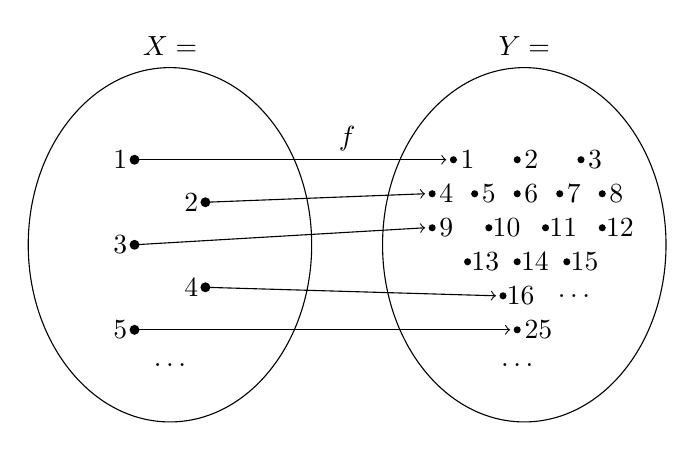
\begin{tikzpicture}[scale=0.9]
%% Mengen:
\draw (0,0) ellipse (2 and 5/2);
\draw (5,0) ellipse (2 and 5/2);
%% linke Menge:
\node at (-0.7,1.2) {$1$};
\fill (-0.5,1.2) circle (0.07);
\node at (0.3,0.6) {$2$};
\fill (0.5,0.6) circle (0.07);
\node at (-0.7,0) {$3$};
\fill (-0.5,0) circle (0.07);
\node at (0.3,-0.6) {$4$};
\fill (0.5,-0.6) circle (0.07);
\node at (-0.7,-1.2) {$5$};
\fill (-0.5,-1.2) circle (0.07);
\node at (0,-1.7) {$\dots$};
%% rechte Menge:
%Erste Zeile:
\fill (4,1.2) circle (0.05); \fill (4.9,1.2) circle (0.05); \fill (5.8,1.2) circle (0.05);
\node at (4.2,1.2) {$1$}; \node at (5.1,1.2) {$2$}; \node at (6,1.2) {$3$};
% Zweite zeile:
\fill (3.7,0.72) circle (0.05); \fill (4.3,0.72) circle (0.05); \fill (4.9,0.72) circle (0.05); \fill (5.5,0.72) circle (0.05); \fill (6.1,0.72) circle (0.05);
\node at (3.9,0.72) {$4$}; \node at (4.5,0.72) {$5$}; \node at (5.1,0.72) {$6$}; \node at (5.7,0.72) {$7$}; \node at (6.3,0.72) {$8$}; 
% Dritte Zeile:
 \fill (3.7,0.24) circle (0.05); \fill (4.5,0.24) circle (0.05); \fill (5.3,0.24) circle (0.05); \fill (6.1,0.24) circle (0.05);
\node at (3.9,0.24) {$9$}; \node at (4.75,0.24) {$10$}; \node at (5.55,0.24) {$11$}; \node at (6.35,0.24) {$12$};
% Vierte Zeile:
\fill (4.2,-0.24) circle (0.05); \fill (4.9,-0.24) circle (0.05); \fill (5.6,-0.24) circle (0.05);
\node at (4.45,-0.24) {$13$}; \node at (5.15,-0.24) {$14$}; \node at (5.85,-0.24) {$15$};
% Fünfte Zeile:
\fill (4.7,-0.72) circle (0.05); \node at (5.7,-0.72) {$\dots$};
\node at (4.95,-0.72) {$16$};
% Sechste Zeile:
\fill (4.9,-1.2) circle (0.05);
\node at (4.9,-1.7) {$\dots$};
\node at (5.2,-1.2) {$25$};
%% Beschriftung:
\node at (2.5,1.5) {$f$};
\node at (0,2.8) {$X=\N$};
\node at (5,2.8) {$Y=\N$};
%% Pfeile:
\draw[->] (-0.5,1.2) -- (3.9,1.2);
\draw[->] (0.5,0.6) -- (3.6,0.72);
\draw[->] (-0.5,0) -- (3.6,0.24);
\draw[->] (0.5,-0.6) -- (4.6,-0.72);
\draw[->] (-0.5,-1.2) -- (4.8,-1.2);
\end{tikzpicture}
\end{center}
\item  
\begin{align*}
 f : \mathbb{R}^2 &\to \mathbb{R}\\
       (x_1,x_2) &\mapsto x_1^2 + x_2^2\\
\end{align*}
\white{4cm}{}
\item
\begin{align*}
 f : \mathbb{Z}\times \mathbb{N} \to \mathbb{Q} \\      
       (q,p) &\mapsto \frac{q}{p}
\end{align*}
\white{4cm}{}
\end{abc}
\end{example}



\subsection*{Well-definedness}
What can go wrong with the definition of a map? 
Sometimes, when defining a function, it is not completely clear, if this makes sense. 
Then one has to work and make this function well-defined. 

\subsubsection{Example: the square-root}

Try to define a map $a \to \sqrt{a}$ in a mathematically rigorous way.

Naive definition:
\begin{align*}
 \sqrt{\hphantom{x}} : \mathbb{R} &\to \mathbb{R}\\
         a &\mapsto \mbox{ the solution of } x^2=a.
\end{align*}
Problem of well-definedness: As we all know, the above equation has two ($a>0$), one ($a=0$), or zero ($a<0$) solutions.

\white{2cm}{}

\emph{First way}: restrict the domain of definition and the codomain
\[
 \mathbb{R}^+_0 =  \{ a \in \mathbb{R}: a \ge 0 \}
\]
Then:
\begin{align*}
 \sqrt{\hphantom{x}} : \mathbb{R}^+_0 &\to \mathbb{R}^+_0\\
         a &\mapsto  \mbox{ the non-negative solution of } x^2=a.
\end{align*}
This yields the classical square-root. 

% \emph{Second way}: invent complex numbers and extend the codomain:
% \begin{align*}
%  \sqrt{} : \mathbb{R} &\to \mathbb{C}\\
%          a &\mapsto \mbox{ the non-negative solution of } x^2=a.
% \end{align*}
% Now there is still a problem: if $a<0$, then we obtain again two solutions 
% $x=\pm i \sqrt{|a|}$ and both are non-negative.
% We have to make the following definition:
% \[
%  P := \{ x \in \mathbb{C} : 0 \le \arg x < \pi \}
% \]
% \begin{align*}
%  \sqrt{} : \mathbb{R} &\to P \\
%          a &\mapsto \mbox{ the solution of } x^2=a \mbox{ in } P
% \end{align*}
% Finally, we can extend our domain even more:
% \begin{align*}
%  \sqrt{} : \mathbb{C} &\to P \\
%          a &\mapsto \mbox{ the solution of } x^2=a \mbox{ in } P,
% \end{align*}
% which is still well defined, as we have seen in the section for complex numbers. 


\subsection*{Image and preimage}

For every well-defined map $f: X\to Y$ and $A\subset X$, $B \subset Y$ we are interested in the following sets:
\begin{Definition}{} 
Let $f: X\rightarrow Y$ be a function
and $A\subset X$ and $B\subset Y$ some sets.

%\begin{figure}[htbp]
  \begin{minipage}[l]{0.5\textwidth}
    \begin{center}
$f(A):= \lbrace f(x): x\in A\rbrace$ \\ is called the \defi{image} 
of $A$ under $f$.
\end{center}
  \end{minipage}
  \begin{minipage}[r]{0.5\textwidth}
  \flushright 
     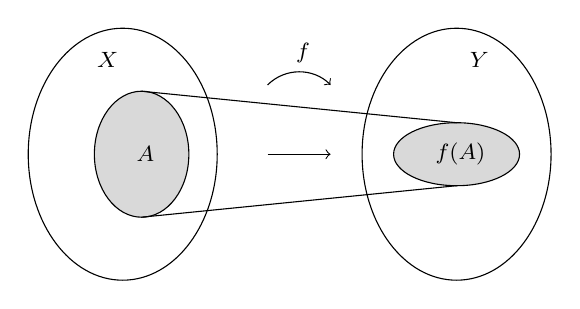
\begin{tikzpicture}[scale=0.8]
% Ellipsen
\draw (-0.3,0) ellipse (3/2 and 2);
\draw (5,0) ellipse (3/2 and 2);
\draw[fill=black!15] (0,0) ellipse (0.75 and 1);
\draw[fill=black!15] (5,0) ellipse (1 and 1/2);
% Pfeile
\draw[->] (2,0) -- (3,0);
\draw (0,1) -- (5,1/2);
\draw (0,-1) -- (5,-1/2);
\draw[->] (2,1.1) to[out=45, in=135] (3,1.1);
% Beschriftungen
\node at (2.5,1.6) {\begin{footnotesize} $f$ \end{footnotesize}};
\node at (-0.6,1.5) {\begin{footnotesize} $X$ \end{footnotesize}};
\node at (5.3,1.5) {\begin{footnotesize} $Y$ \end{footnotesize}};
\node (A) at (0,0) {\begin{footnotesize} $A$ \end{footnotesize}};
\node (B) at (5,0) {\begin{footnotesize} $f(A)$ \end{footnotesize}};
\end{tikzpicture}
  \end{minipage}
%\end{figure}

~\\

%\begin{figure}[htbp]
  \begin{minipage}[l]{0.5\textwidth}
    \begin{center}
    $f^{-1}(B):= \lbrace x\in X: f(x) \in B \rbrace$ \\ is called
    the \defi{preimage} of $B$ under $f$.
\end{center}
  \end{minipage}
  \begin{minipage}[r]{0.5\textwidth}
  \flushright
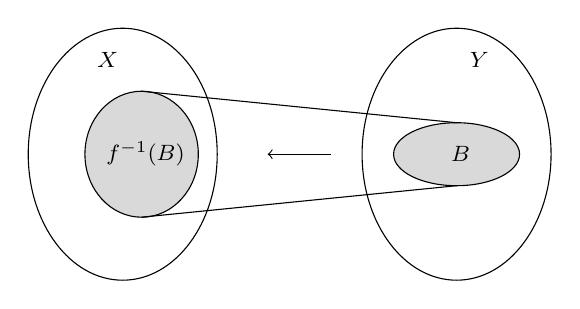
\begin{tikzpicture}[scale=0.8]
% Ellipsen
\draw (-0.3,0) ellipse (3/2 and 2);
\draw (5,0) ellipse (3/2 and 2);
\draw[fill=black!15] (0,0) ellipse (0.9 and 1);
\draw[fill=black!15] (5,0) ellipse (1 and 1/2);
% Pfeile
\draw[<-] (2,0) -- (3,0);
\draw (0,1) -- (5,1/2);
\draw (0,-1) -- (5,-1/2);
%\draw[->] (2,1.1) to[out=45, in=135] (3,1.1);
% Beschriftungen
\node at (2.5,1.6) {\begin{footnotesize}  \end{footnotesize}};
\node at (-0.6,1.5) {\begin{footnotesize} $X$ \end{footnotesize}};
\node at (5.3,1.5) {\begin{footnotesize} $Y$ \end{footnotesize}};
\node (A) at (0,0) {\begin{footnotesize} $f^{-1}(B)$ \end{footnotesize}};
\node (B) at (5,0) {\begin{footnotesize} $B$ \end{footnotesize}};
\end{tikzpicture}
  \end{minipage}
%\end{figure}
\end{Definition}
%
\white{3cm}{
Note that the preimage can also be the empty set if none of the
elements in $B$ are ``hit'' by the map.

To describe the behaviour of a map,
the following sets are very important:
}
\begin{Definition}{Range and fiber}
Let $f: X\rightarrow Y$ be a map. Then
\begin{align*}
 \mathrm{Ran}(f) &:= f(X) = \{ f(x) : x \in X \} ~\text{ is called the \defi{range} of} \text{ }f.
\end{align*}
%and if there is $0 \in Y$, then 
%\begin{align*}
% f^{-1}(\{0\}) = \mathrm{Kern}\, &= \{ x : f(x) = 0 \} &\defi{kernel} \text{ or } \defi{nullspace} \text{ }f\\
%\end{align*}
For each $y\in Y$ the set
\begin{align*}
 f^{-1}(\{y \}) &:= \{ x \in X : f(x) = y \} ~ \mbox{ is called a \defi{fiber} of }  f.
\end{align*}
\end{Definition}

If these definitions seem too abstract, the following video may help
you to get used to the terms.

\begin{Video}{Range{,} Image and Preimage}
	\begin{minipage}{0.5\linewidth}
		\begin{center}
			\includegraphics[width=0.9\linewidth]{pics/SLS5.png}
		\end{center}
	\end{minipage}
	%
	\begin{minipage}{0.5\linewidth}
		\begin{center}
			\url{https://jp-g.de/bsom/la/sls5/}
			\includegraphics[width=0.4\linewidth]{pics/qr-code_sls5.pdf}
		\end{center}
	\end{minipage}
\end{Video}


\subsection*{Injectivity, surjectivity, bijectivity, inverse}

\begin{Definition}{Injective{,} surjective and bijective}
A map $f: X \to Y$ is called
\begin{itemize}
 \item \defi{injective} if every fiber of $f$ has only one element: $x_1 \neq x_2 \Rightarrow f(x_1) \neq f(x_2)$.
 \item \defi{surjective} if $\mathrm{Ran}(f)=Y$. With quantifiers: $\forall y\in Y~ \exists x\in X \,:\, f(x)=y$.
 \item \defi{bijective} if $f$ is both injective and surjective.
\end{itemize}
\end{Definition}


\begin{example}
Define the function that maps each student to
her or his chair. This means that $X$ is the set of all students in the room,
and $Y$ the set of all chairs in the room.
\white{6cm}{
\begin{itemize}
 \item well-defined: every student has a chair
 \item surjective: every chair is taken
 \item injective: on each chair there is no more than one student
 \item bijective: every student has his/her own chair, and no chair is empty
\end{itemize}
}
\end{example}


\begin{center}
     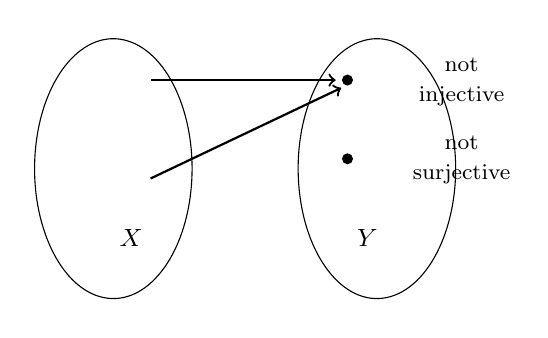
\begin{tikzpicture}[scale=1]
% Mengen
\draw (0,0)  arc[x radius = 1, y radius = 1.65, start angle= 80, end angle= 440];
\draw (3,0)  arc[x radius = 1, y radius = 1.65, start angle= 100, end angle=460];
% Punkte
\fill (2.8,-0.5) circle (0.07);
\fill (2.8,-1.5) circle (0.07);
% Beschriftung
\node at (4.2,-0.3) {\begin{footnotesize} not \end{footnotesize}};
\node at (4.2,-0.7) {\begin{footnotesize} injective \end{footnotesize}};
\node at (4.2,-1.3) {\begin{footnotesize} not \end{footnotesize}};
\node at (4.2,-1.7) {\begin{footnotesize} surjective \end{footnotesize}};
\node at (0,-2.5) {\begin{small} $X$ \end{small}};
\node at (3,-2.5) {\begin{small} $Y$ \end{small}};
% Pfeile
\draw[->, thick] (0.3,-0.5) -- (2.65,-0.5);
\draw[->, thick] (0.3,-1.75) -- (2.72,-0.6);
\end{tikzpicture}
\end{center}



\begin{Faust}{Surjective{,} injective{,} bijective}
A map  $f: X \rightarrow Y$ is
\begin{align*}
\text{surjective}\ &\Leftrightarrow\ \text{at each $y\in Y$ arrives {\textbf{at least}} one arrow} \\
&\Leftrightarrow\ f(X)=Y\\
&\Leftrightarrow\ \text{the equation $f(x)=y$ has for all $y\in Y$ a solution} \\
\\
\text{injective}\ &\Leftrightarrow\ \text{at each $y\in Y$ arrives {\textbf{at most}} one arrow}\\
&\Leftrightarrow\ \left( x_1 \neq x_2\quad \Rightarrow\quad f(x_1)\neq f(x_2) \right) \\
&\Leftrightarrow\ \left( f(x_1)=f(x_2)\quad \Rightarrow\quad x_1=x_2 \right) \\
&\Leftrightarrow\ \text{the equation $f(x)=y$ has for all $y\in f(X)$ 
a \textbf{unique} solution} \\
\\
\text{bijective}\ &\Leftrightarrow\ \text{at each $y\in Y$ arrives {\textbf{exactly}} one arrow} \\
&\Leftrightarrow\ \text{the equation $f(x)=y$ has for all $y\in Y$
a \textbf{unique} solution}
\end{align*}
\end{Faust}



%
%
%Application: Solution of equations: $f(x)=y$:
%\begin{align*}
% f &\mbox{ injective : if a solution exists, then it is unique}\\
% f &\mbox{ surjective : a solution always exists, but need not be unique}\\
% f &\mbox{ bijective : a solution always exists, and is unique}
%\end{align*}






Thus, if $f$ is bijective, there is a well defined inverse map 
\begin{align*}
f^{-1}:Y&\to X\\
       y &\mapsto x \text{ where } f(x)=y \,.
\end{align*}
Then $f$ is called \defi{invertible}
and $f^{-1}$ is called the \defi{inverse map} of $f$.

\white{3cm}{}


\begin{example}{} \label{Bsp:Umkehrabbildung}
Consider the function $f: \N \rightarrow \{1, 4, 9, 16, \ldots\}$
given by $f(n) = n^2$. This is a bijective function.
The inverse map $f^{-1}$ is given by:
\begin{align*}
f^{-1}:\lbrace1,4,9,16,25,\dots \rbrace &\rightarrow \N \\
m & \mapsto \sqrt{m} \\
\text{or: } n^2 &\mapsto n
\end{align*}
\begin{center}
     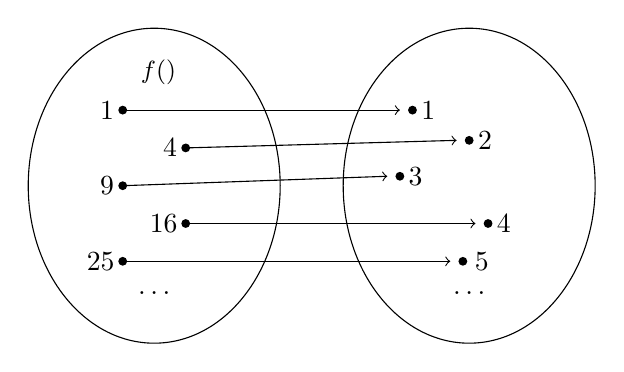
\begin{tikzpicture}[scale=0.8]
%% Mengen:
\draw (0,0) ellipse (2 and 5/2);
\draw (5,0) ellipse (2 and 5/2);
%% linke Menge:
\node at (-0.75,1.2) {$1$};
\fill (-0.5,1.2) circle (0.07);
\node at (0.25,0.6) {$4$};
\fill (0.5,0.6) circle (0.07);
\node at (-0.75,0) {$9$};
\fill (-0.5,0) circle (0.07);
\node at (0.15,-0.6) {$16$};
\fill (0.5,-0.6) circle (0.07);
\node at (-0.85,-1.2) {$25$};
\fill (-0.5,-1.2) circle (0.07);
\node at (0,-1.7) {$\dots$};
%% rechte Menge:
\fill (4.1,1.2) circle (0.07); 
\node at (4.35,1.2) {$1$}; 
\fill (5,0.72) circle (0.07); 
\node at (5.25,0.72) {$2$}; 
 \fill (3.9,0.15) circle (0.07); 
\node at (4.15,0.15) {$3$}; 
\fill (5.3,-0.6) circle (0.07); 
\node at (5.55,-0.6) {$4$};
\fill (4.9,-1.2) circle (0.07);
\node at (5.2,-1.2) {$5$};
\node at (5,-1.7) {$\dots$};
%% Beschriftung:
\node at (0,1.8) {\begin{small} $f(\N)$ \end{small}};
\node at (5,1.8) {\begin{small} $\N$ \end{small}};
%% Pfeile:
\draw[->] (-0.5,1.2) -- (3.9,1.2);
\draw[->] (0.5,0.6) -- (4.8,0.72);
\draw[->] (-0.5,0) -- (3.7,0.15);
\draw[->] (0.5,-0.6) -- (5.1,-0.6);
\draw[->] (-0.5,-1.2) -- (4.7,-1.2);
\end{tikzpicture}
\end{center}
%Man beachte, dass der Definitionsbereich von $f^{-1}$ nicht ganz $\N$ ist sondern nur $f(\N)$, also die Menge der Quadratzahlen.
\end{example}


\white{2cm}{}



\begin{example}
For a function $f:\R\rightarrow\R$, we can sketch the graph $\lbrace(x,f(x)): x\in X\rbrace$ in the $x$-$y$-plane:
\begin{figure}[htbp]
  \begin{minipage}[b]{0.5\textwidth}
   \centering
    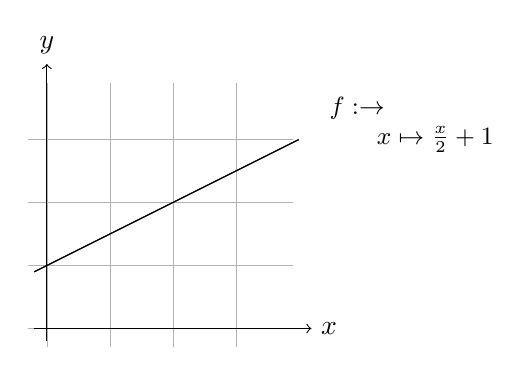
\begin{tikzpicture}[scale=0.8, domain=-0.2:4] % Zeichenbereich
% Gitter
\draw[very thin,color=black!30] (-0.3,-0.3) grid (3.9,3.9);
% Achsen
\draw[->] (-0.2,0) -- (4.2,0) node[right] {$x$};
\draw[->] (0,-0.2) -- (0,4.2) node[above] {$y$};
% Funktionen
\draw plot[samples=300] (\x,\x/2+1) node[right] at (4.2,3.5) {\begin{small} $f: \R \rightarrow \R$ \end{small}};
\draw plot[samples=300] (\x,\x/2+1) node[right] at (4.95,3) {\begin{small} $x \mapsto \frac{x}{2}+1$ \end{small}};
\end{tikzpicture}
  \end{minipage}
  \begin{minipage}[b]{0.5\textwidth}
  \centering
    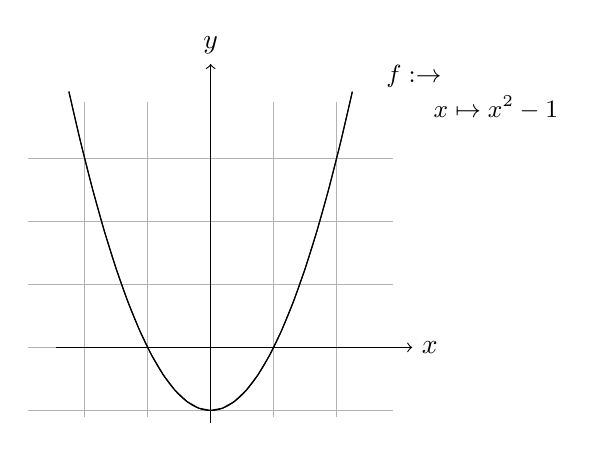
\begin{tikzpicture}[scale=0.8, domain=-2.25:2.25] % Zeichenbereich
% Gitter
\draw[very thin,color=black!30] (-2.9,-1.1) grid (2.9,3.9);
% Achsen
\draw[->] (-2.45,0) -- (3.2,0) node[right] {$x$};
\draw[->] (0,-1.2) -- (0,4.5) node[above] {$y$};
% Funktionen
\draw plot[samples=300] (\x,\x*\x-1) node[right] at (2.5,4.3) {\begin{small} $f: \R \rightarrow \R$ \end{small}};
\draw plot (\x,\x*\x-1) node[right] at (3.25,3.8) {\begin{small} $x \mapsto x^2-1$ \end{small}};
\end{tikzpicture}
  \end{minipage}
\end{figure}
\begin{center}
     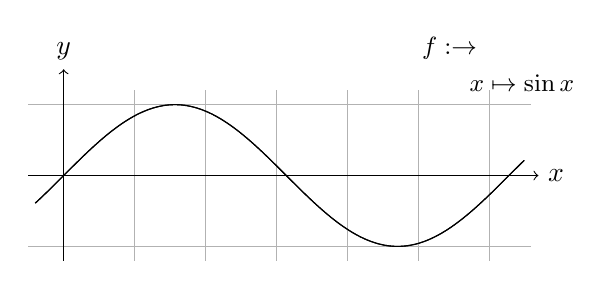
\begin{tikzpicture}[scale=0.9, domain=-0.4:6.5] % Zeichenbereich
% Gitter
\draw[very thin,color=black!30] (-0.5,-1.2) grid (6.6,1.2);
% Achsen
\draw[->] (-0.5,0) -- (6.7,0) node[right] {$x$};
\draw[->] (0,-1.2) -- (0,1.5) node[above] {$y$};
% Funktionen
\draw plot[samples=300] (\x,{sin(\x r)}) node[right] at (4.8,1.8) {\begin{small} $f: \R \rightarrow \R$ \end{small}};
\draw plot[samples=300] (\x,{sin(\x r)}) node[right] at (5.47,1.3) {\begin{small} $x \mapsto \sin x$ \end{small}};
\end{tikzpicture}
\end{center}
Which of the functions are injective, surjective or bijective?
\end{example}


These notions might seem a little bit off-putting, but we will use them so often that you need to get use to them. Maybe the following video
helps you as well:

\begin{Video}{Injectivity{,} Surjectivity and Bijectivity}
	\begin{minipage}{0.5\linewidth}
		\begin{center}
			\includegraphics[width=0.9\linewidth]{pics/SLS6.png}
		\end{center}
	\end{minipage}
	%
	\begin{minipage}{0.5\linewidth}
		\begin{center}
			\url{https://jp-g.de/bsom/la/sls6/}
			\includegraphics[width=0.4\linewidth]{pics/qr-code_sls6.pdf}
		\end{center}
	\end{minipage}
\end{Video}



\subsection*{Composition of maps}

\begin{Definition}{}
If $f:X \to Y$ and $g : Y\to Z$, we may compose, or concatenate these maps:
\begin{align*}
 g \circ f : X &\to  Z\\
            x &\mapsto g(f(x))
\end{align*}
We call $g \circ f$ the \defi{composition} of the two functions.
\end{Definition}

Usually, $g\circ f \neq f\circ g$, the latter does not even make sense, in general. 
\[
 X \to Y \to Z
\]

\begin{center}
  \centering
     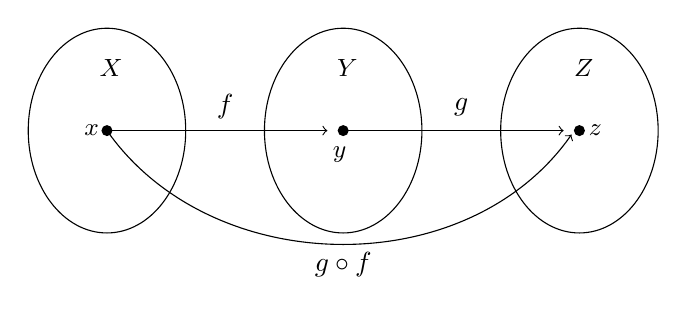
\begin{tikzpicture}[scale=1]
\draw (0,0) ellipse (1 and 1.3);
\draw (3,0) ellipse (1 and 1.3);
\draw (6,0) ellipse (1 and 1.3);
\fill (0,0) circle (0.07);
\node at (-0.25,0) {\begin{small} $x$ \end{small}};
\fill (3,0) circle (0.07);
\node at (2.9,-0.3) {\begin{small} $y$ \end{small}};
\fill (6,0) circle (0.07);
\node at (6.15,0) {\begin{small} $z$ \end{small}};

\node at (1.5,0.3) {$f$};
\node at (0,0.8) {\begin{small} $X$ \end{small}};
\node at (3,0.8) {\begin{small} $Y$ \end{small}};
\draw[->] (0,0) -- (2.8,0);
\node at (4.5,0.3) {$g$};
\node at (6,0.8) {\begin{small} $Z$ \end{small}};
\draw[->] (3,0) -- (5.8,0);
\draw[->] (0,0) to[out=-55, in=-125] (5.9,-0.05);
\node at (3,-1.7) {$g \circ f$};
\end{tikzpicture}
\end{center}




\begin{example}{} \label{Bsp:Komposition}
%\begin{enumerate}[\bf a)]
\begin{abc}
%\itemsep0.7mm
\item $f: \R \rightarrow \R$, $x\mapsto x^2$;~ $g:\R \rightarrow \R$, $x\mapsto \sin(x)$
\begin{align*}
g\circ f: \R &\rightarrow \R \\
x &\mapsto \sin(x^2) \\
f\circ g: \R &\rightarrow \R \\
x &\mapsto (\sin(x))^2
\end{align*}
\item Let $X$ be a set. Then $\id_X: X\rightarrow X$ with $x\mapsto x$ is called the \defi{identity map}.
If there is no confusion, one usually writes $\id$ instead of $\id_X$. 
Let $f: X\rightarrow X$ be a function. Then
\[
f\circ \id=f=\id\circ f.
\]
\end{abc}
\white{40mm}{}
%\end{enumerate}
\end{example}




\VL{2}



\white{}{
\subsection*{Algebraic vs. analytic properties of maps}

Maps are a versatile tool in mathematics and often the main object of interest. Many other problems can be
reformulated with maps. 

We have seen here some \emph{algebraic} properties: injectivity, surjectivity, bijectivity.

Other algebraic properties may be compatibility with operations on $X$ and $Y$. 

Examples:
\begin{align*}
 f(x-y) &= f(x)-f(y)  &\mbox{ affine maps }\\
 f(\alpha x) &= \alpha f(x)  &\mbox{ homogenous maps }\\
 f(\alpha x+\beta y) &= \alpha f(x)+\beta f(y)  &\mbox{ linear maps }\\
 f(x y) &= f(x) f(y) \dots 
\end{align*}
These are sometimes called ''homomorphisms``. 

In analysis next semester, we will learn about other properties, like continuity, differentiability, integrability, $\dots$
But for this, we have to define \emph{open sets} first. 
}

